\documentclass[12pt,letterpaper]{report} % a4paper

% packages
\usepackage{graphicx}

% variables
\newcommand{\picSize}{0.19\textwidth}
\newcommand{\textSize}{0.79\textwidth}

% define the title
\title{Open Data Lab Annual Report - 2018}
\author{The Open Data Lab Collaboration}

%%% ---ooo000 END PREAMBLE 000ooo---

\begin{document}

% generates the title
\maketitle

% introduction
% include content
\chapter*{The Team}  \begin{tabular}[t]{lp{\textSize}}
\hline
\hline

\raisebox{-0.84\totalheight}{
\includegraphics[width=\picSize]{images/people/alonzi.png}}
& 
\begin{tabular}[t]{p{\textSize}}
$\mathbf{Pete\:Alonzi}$ came to data science by way of the particle physics community. As a result he has great interest in making data open and usable to broad audiences. He sereves as a data scientist at the DSI and is the project manager for the Open Data Lab.
\end{tabular}
\\\hline

\raisebox{-0.84\totalheight}{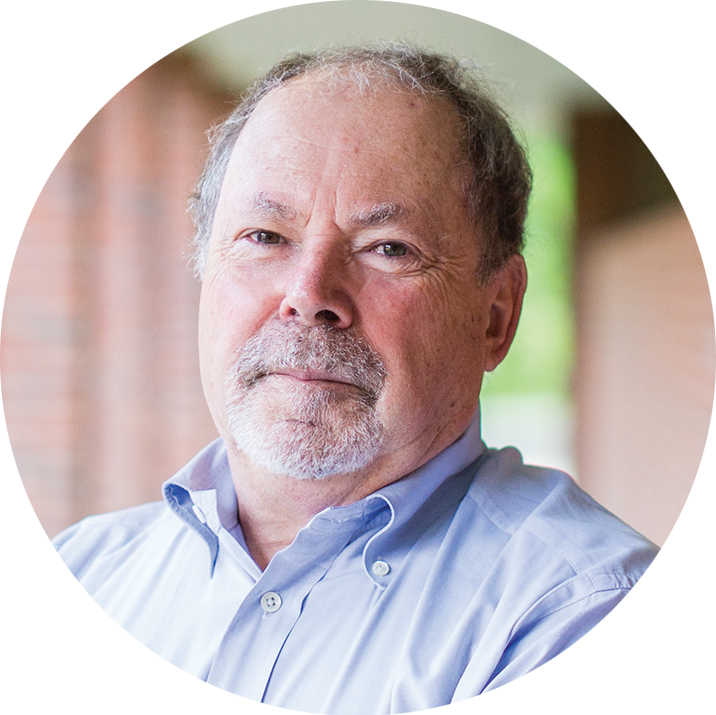
\includegraphics[width=\picSize]{images/people/bourne.png}}
 & 
 \begin{tabular}[t]{p{\textSize}}
$\mathbf{Phil\:Bourne}$ "At vero eos et accusamus et iusto odio dignissimos ducimus qui blanditiis praesentium voluptatum deleniti atque corrupti quos dolores et quas molestias excuri sint occaecati cupiditate non provident,At vero eos et accusamus et dent, " 
\end{tabular}
\\\hline

\raisebox{-0.84\totalheight}{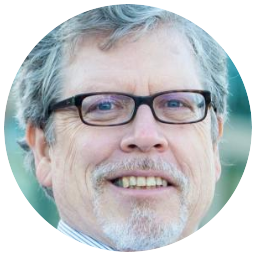
\includegraphics[width=\picSize]{images/people/clark.png}}
 & 
 \begin{tabular}[t]{p{\textSize}}
$\mathbf{Tim\:Clark}$ "Tim Clark, Ph.D., is a biomedical informatician and computer scientist with 28 years experience in academic, government and industry.  He is an expert in biomedical knowledge representation, data fusion and open science applications. He is an Associate Professor appointed in the UVA School of Medicine \& the Data Science Institute." 
\end{tabular}
\\\hline

\raisebox{-0.84\totalheight}{\includegraphics[width=\picSize]{images/people/levinson.png}}
 & 
 \begin{tabular}[t]{p{\textSize}}
$\mathbf{Max\:Levinson}$ "Max Levinson is a  Software Engineer and Cloud Developer within Public Health Services. When not building out REST apis for the NIH Data Commons Project, he can be found hacking on the Open Data Lab Project.

Max is passionate about microservices development, knowledge graphs, and anything python." 
\end{tabular}
\\\hline

\raisebox{-0.84\totalheight}{
\includegraphics[width=\picSize]{images/people/mietchen.png}}
 & 
 \begin{tabular}[t]{p{\textSize}}
$\mathbf{Daniel\:Mietchen}$ "At vero eos et accusamus et iusto odio dignissimos ducimus qui blanditiis praesentium voluptatum deleniti atque corrupti quos dolores et quas molestias excuri sint occaecati cupiditate non provident,At vero eos et accusamus et dent, " 
\end{tabular}
\\\hline

\raisebox{-0.84\totalheight}{
\includegraphics[width=\picSize]{images/people/rasberry.png}}
 & 
 \begin{tabular}[t]{p{\textSize}}
$\mathbf{Lane\:Rasberry}$ "At vero eos et accusamus et iusto odio dignissimos ducimus qui blanditiis praesentium voluptatum deleniti atque corrupti quos dolores et quas molestias excuri sint occaecati cupiditate non provident,At vero eos et accusamus et dent, " 
\end{tabular}
\\

\hline
\hline
\end{tabular}

% \smash{...} to override bounding
 % People working on project, alphabetical

\chapter*{Letter from the editor}  
hello world

 % Mission and vision and philosophy

% insert the table of contents
\tableofcontents
\pagebreak

\chapter{Overview} \section{What is the Open Data Lab?}
\subsection{Long Term Goals}
\subsection{Short Term Goals}
\section{A phased approach}
\section{The team}
\section{User archetypes}
\section{What's next for the Open Data Lab?}


\chapter{Key Developments} \section{Phase 1 - Closed $\beta$}
\section{Establishment of User base}
\section{Technology exploration}
\subsection{Amazon Web Services}
\subsection{Local UVA - Rivanna and Ivy}
\subsection{Github}
\subsection{Dataverse}

\chapter{Datasets} \section{Healthy Markets}
\section{Numismatic}

\chapter{Research} \section{Research Projects}
\section{Datasets}


\chapter{Education} innovative workshop using sagemaker and jupyter hub

\chapter{Vital Metrics} \section{AWS usage}
\section{FTE analysis}
\section{Budget}

%\chapter{publications}

\end{document}




% I view ‘open’ broadly. Open means: accessible, useable, and responsible. Whatever the context, be it data, methods, education, or even lavatories, accessibility and usability are essential for openness. However just as essential is the responsibility. That may take the form of ethical responsibility, scientific responsibility, financial responsibility, educational responsibility, and the list goes on. By necessity this means, open does not imply free. The burden of responsibility lies both with the producer and the consumer. Which means that open means community. Open means culture. Both of these states are not free but they are empowering and well worth the price of openness.
